% g2_01 (Volkov string 2; 1-5, 3-4: self-energy graph) drawn as a vertex "triangle".
% External photon q at the top apex (vertex 2); electron line enters bottom left, leaves bottom right, 120 degrees apart.
% x0..x3: electron segments 1-2, 2-3, 3-4, 4-5; x4: photon 1-5 (Cheng-Wu fixes x4 = 1); x5: self-energy photon 3-4.
% Unlabelled; arrowheads 1.2x those of twoloop_diagrams.tex.  pdflatex g2_01_triangle.tex
\documentclass{article}
\usepackage{tikz}
\usetikzlibrary{decorations.pathmorphing,decorations.markings}
\tikzset{
  photon/.style={decorate,decoration={snake,amplitude=0.6mm,segment length=2mm,pre length=0.3mm,post length=0.3mm}},
  fermion/.style={thick,postaction={decorate},decoration={markings,mark=at position 0.55 with {\arrow[scale=1.2]{stealth}}}},
  vtx/.style={circle,fill,inner sep=1pt},
  lab/.style={font=\small},
  num/.style={font=\scriptsize,text=gray},
}
\hoffset=-1in \voffset=-1in \parindent=0pt \pagestyle{empty}
\newsavebox\diag
\newcommand\onepage[1]{\sbox\diag{#1}\pdfpagewidth=\wd\diag \pdfpageheight=\dimexpr\ht\diag+\dp\diag\relax
  \shipout\hbox{\raise\dp\diag\box\diag}}
\begin{document}
\onepage{%
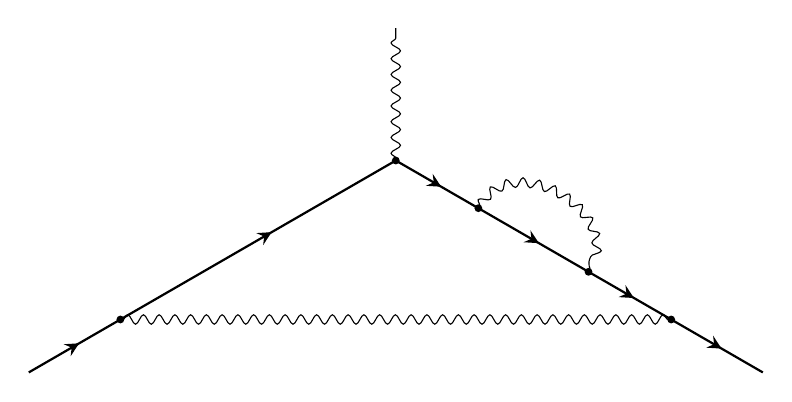
\begin{tikzpicture}[scale=1.4]
  % apex (vertex 2) at the top, electron lines at 120 degrees; self-energy ends 20% further apart than
  % in the first version (1/3 and 2/3 of the leg), same arc height.  No labels (vertex order 1..5 along the line).
  \coordinate (in) at (-3.329,-1.922);  \coordinate (out) at (3.329,-1.922);
  \coordinate (v1) at (-2.498,-1.442);  \coordinate (v2) at (0,0);
  \coordinate (v3) at (0.749,-0.4325);  \coordinate (v4) at (1.748,-1.0095);  \coordinate (v5) at (2.498,-1.442);
  \draw[fermion] (in) -- (v1);
  \draw[fermion] (v1) -- (v2);
  \draw[fermion] (v2) -- (v3);
  \draw[fermion] (v3) -- (v4);
  \draw[fermion] (v4) -- (v5);
  \draw[fermion] (v5) -- (out);
  \draw[photon] (v1) -- (v5);
  \draw[photon] (v3) .. controls (1.049,0.0875) and (2.048,-0.4895) .. (v4);
  \draw[photon] (v2) -- (0,1.2);
  \foreach \i in {1,...,5} \node[vtx] at (v\i) {};
\end{tikzpicture}}
\end{document}
